\documentclass[10pt,draftclsnofoot,onecolumn]{IEEEtran}
\usepackage{pdfpages}
\usepackage{lipsum}
\usepackage[utf8]{inputenc}
\usepackage[T1]{fontenc}
\usepackage{geometry}
\usepackage{setspace}
\usepackage{graphicx}
\renewcommand{\maketitle}{\bgroup\setlength{\parindent}{0pt}
\begin{flushleft}
\Huge
  \textbf{\@Multi-Camera Stereoscopic Vision: \\Winter Progress Report}
\large
\vspace{3mm}\\
  Erin Sullens, John Miller, Sam Schultz \\
   \vspace{3mm}
  CS461

Winter 2017

Group 54

Sponsor: Kevin McGrath

Group Name: ImMaculaTe Vision
  
\end{flushleft}\egroup
}
\renewcommand{\familydefault}{\sfdefault}
\usepackage[document]{ragged2e}
\geometry{letterpaper, margin=0.75in}
\newcommand\tab[1][1cm]{\hspace*{#1}}
\title{}
\author{ }

\date{October 2016}
\begin{document}
\singlespacing
%\fontfamily{lmss}\selectfont
%\begin{flushleft}
\maketitle
%\end{flushleft}
\begin{center}



\vspace{2in}
{\Medium\textbf{Abstract}}
\end{center}
\setlength{\parindent}{0cm}

This document is a progress report that talks about what we accomplished this term, any problems that we ran into, and what we still need to accomplish.  \\

\begin{document}
\newpage
{\Large\textbf{1 Project Purposes and Goals}}\\
  \vspace{5mm}
 In this project, take footage from road trips and convert them into a stereoscopic 3D video format that can be viewed on a VR headset such as an OSVR headset. A desktop and mobile application will be created and used to process the videos and convert them into the correct format. This could be used just for entertainment purposes, but there are other applications as well. Indoor bicycle training could feel much like biking in the wilderness if the cyclist wears a VR headset and is able to view a road trip in 3D. Our client's main motivation for this project is to be able to re-live his road trips in 3D virtual reality.  \\
   \vspace{5mm}
{\Large\textbf{2 Erin's Progress (Authorship: Erin Sullens)}}\\
  \vspace{5mm}
  The three requirements that I am responsible for in this project are video stabilization, video cropping, and parsing the BLOB file that the Garmin cameras output. \\
  \vspace{5mm}
{\Large\textbf{2.1 Where I am currently in the project: }}\\
  \vspace{5mm}

In this term, I have been working mostly on the video stabilization requirement, and the video cropping requirement. Over winter break, I found a piece of code that stabilizes and crops video, but it didn't work right away on my computer, mostly because OpenCV wasn't working on my Mac, or my PC. It took me awhile to get OpenCV working, but when it did, the code ran just fine. In the code, you can specify the smoothing radius, which I have set to 30, and you can specify the pixels to crop on the top and bottom of the video.  \\
\vspace{5mm}
\begin{figure}[h!]
  
  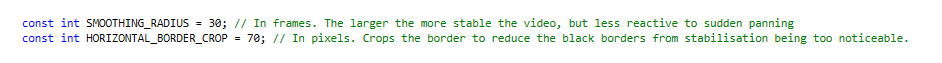
\includegraphics[scale=.7]{pic1}
  \caption{The code for specifying smoothing radius and border crop [2]}
\end{figure}\\
 \vspace{5mm}
 The stabilization that this code provides will definitely be sufficient for the types of videos that our client will be using. The video that I have been using as a test for this code is much more unstable than the videos that the Garmin cameras will produce from being mounted to the front of a vehicle. \\
  \vspace{5mm}
  
As far as cropping the videos to get rid of the black lines created by the stabilization process, this code will also work. The two images below show the same frame, one that has the border crop set to 20, and the other has the border crop set to 100. We will probably need a border crop somewhere in between, but I chose 100 to make the difference obvious. \\
\vspace{5mm}
\begin{figure}[h!]
  
  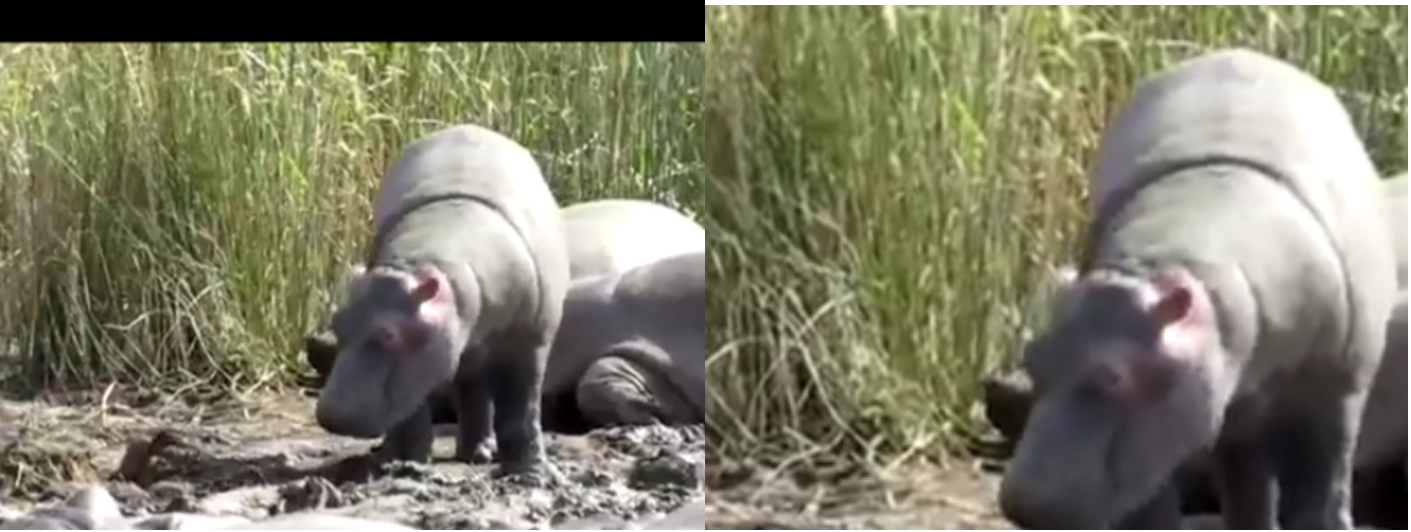
\includegraphics[scale=.5]{pic2}
  \caption{On the left, the image is cropped by 20 pixels, and on the right the image is cropped by 100 pixels. }
\end{figure}\\
\vspace{5mm}
Another part of this code that is important is where it outputs the resulting stabilized video. Instead of creating a video, it instead outputs images of all of the frames.\\
\vspace{5mm}
\begin{figure}[h!]
  
  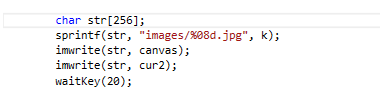
\includegraphics[scale=1]{pic3}
  \caption{Code that outputs the resulting images [2] }
\end{figure}\\
\vspace{5mm}
The other requirement that I have spent a little bit of time on, is the BLOB parser. None of the technologies that I researched last term for the technology review have worked, and Kevin has not been able to contact Garmin about obtaining a parser from them, so we have been looking around for another parser that might work. Once we realized that the BLOB file is a fit file, we were able to narrow down our research, and have found one SDK by ANT that works perfectly [1]. There were a few problems with it at the beginning, but Sam messed around with it for a few days and got it to work eventually. \\
\vspace{20mm}
{\Large\textbf{2.2 What I have left to do }}\\
\vspace{5mm}
For my requirements, which include stabilization of video, cropping the video, and parsing the BLOB files, the only things I have left to do are creating a video from the images that stab.cpp outputs.. Once that piece is working, the only thing our group has left to do is combine all of the requirements into the desktop app and the mobile app, and take care of any bugs that come up in the process. Getting the mobile app working might be difficult since mobile devices have limited storage and since we are needing to handle such large video files, that might end up being a problem. \\
\vspace{5mm}
{\Large\textbf{2.3 Problems that have come up}}\\
\vspace{5mm}
One problem that came up in the beginning was getting OpenCV working on my computer, like I mentioned before. I have been using Visual Studio for running the stabilization and cropping code, and it was having a hard time accessing the OpenCV libraries that I installed on my computer. However, after watching multiple YouTube videos on how to configure Visual Studio for running OpenCV, I was finally able to get it to work properly. 
\vspace{5mm}
The other problem I have run into was getting a BLOB parser to work, but Sam was able to find one that works, so now we access the metadata from the cameras. \\
\vspace{5mm}
{\Large\textbf{3 Sam's Progress (Authorship: Sam Schultz)}}\\

\vspace{5mm}
{\Large\textbf{3.1 Where I am currently in the project: }}\\
\vspace{5mm}
The main components that I have worked on thus far in the term are the combination of the 2 video files into the correct format to display on the VR device. I have created a program that reads in the 2 video files and combines them into a side-by-side format that will display each video onto each eye which creates the stereoscopic effect. I have successfully used OpenCV to create the solution to this problem using the c++ classes provided by the framework. At this point in development no multiple viewing angles has been set up (think 360 degree video). I also have been helping Erin get the FitParse solution to work correctly using the Ant - Garmin Fit file SDK [1]. At this point in development I have not started the frame correlation validation process because the FitParse solution using the sdk proved to be a very difficult roadblock and was necessary to have completed before we could use the parsed fit file information to validate the video files. At this point in time we have successfully parsed to fit file using the SDK to retrieve information and we are currently working on formatting the output to file which will then be used by my to be created validation script which will use the information to prove that the videos are taken at the same time and same place.\\
\vspace{5mm}
\begin{figure}[h!]
  
  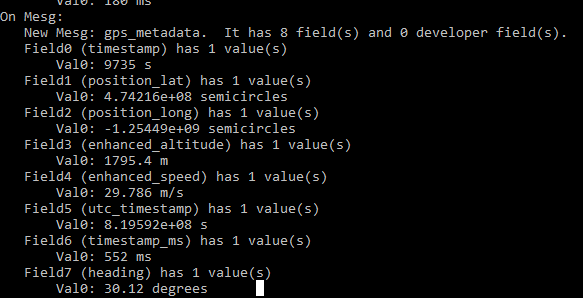
\includegraphics[]{pic6}
  \caption{An example of the FitParse output GPS metadata record displayed in the console window }
\end{figure}\\
\vspace{5mm}
\begin{figure}[h!]
  
  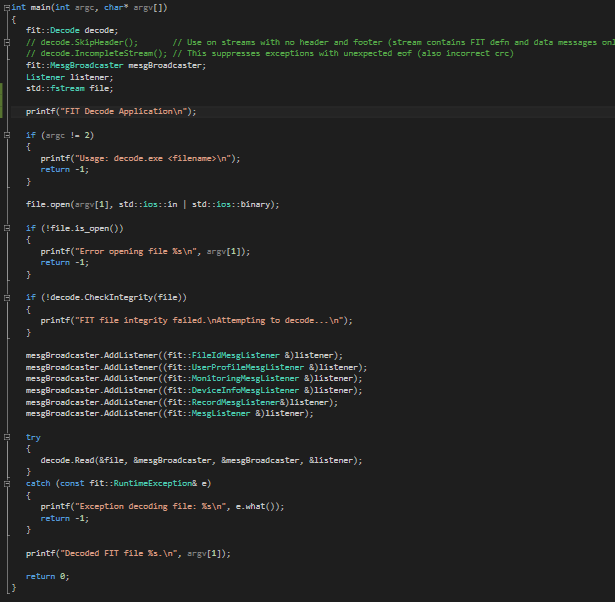
\includegraphics[scale=.8]{pic7}
  \caption{This is the current program that takes the fit file as input and outputs to the console window as seen in Figure 4 }
\end{figure}\\
\vspace{5mm}
The next step to clean up the output is to modify the mesgBroadcaster class to only include the listeners for only the GPS metadata and write it to a file instead of the console window.\\
\vspace{5mm}
{\Large\textbf{3.2 Problems that have come up}}\\
\vspace{5mm}
The problems that I have ran into with helping Erin get the Blob parser to work include the configuration process of the application. When I initially tried to get the SDK to run I was receiving compile time errors that prevented the object files from being created. The solution that I found to get passed this problem was to compile the sdk on a lower warning level. Initially it was treating all warnings as errors but when I disabled this component the project compiled and successfully output the GPS metadata that we need to create the validation program which I am now able to start on. With our current setup of the BLOB parsing application it took 123 minutes to parse and out to the console window on a 32 MB fit file. We are currently working on reducing this run time. At this point in time I have only had time to perform one successful parse of a file, however I have some ideas for future runs to reduce the overall run time of the program. I will try running it in release mode instead of debug mode as well as clean up the mesgListeners for the records that it outputs which will create a cleaner and hopefully only relevant output information.\\
\vspace{5mm}
\begin{figure}[h!]
  
  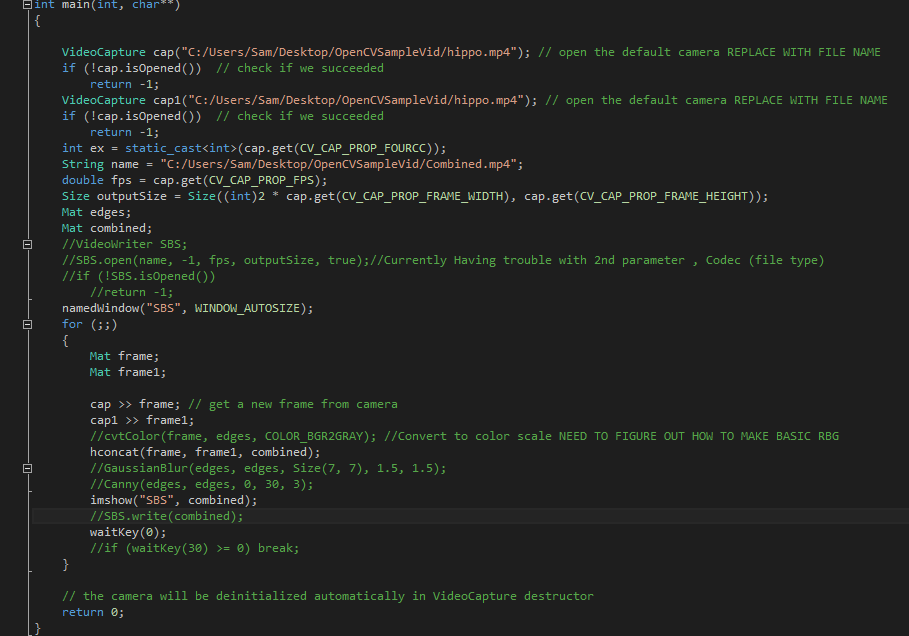
\includegraphics[scale=.5]{pic4}
  \caption{A code snippet of the solution to combine the multiple video files into the side-by-side format. This  code takes in two video files and creates a new video that has the ability to fine tune the resolution, FPS, and file output type }
\end{figure}\\
\vspace{5mm}
\begin{figure}[h!]
  
  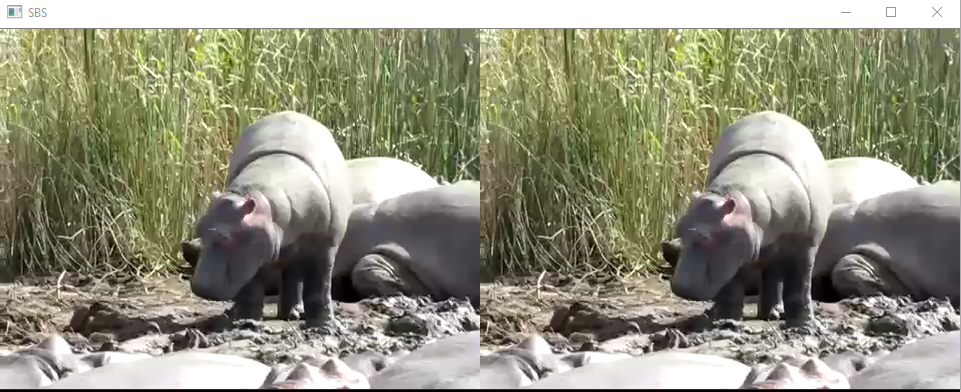
\includegraphics[scale=.6]{pic5}
  \caption{An example of the side-by-side format produced by the code in Figure 6 }
\end{figure}\\
\vspace{5mm}
Current issues with the script above include writing the combined video to file. The roadblock lies within the codec portion of the VideoWriter constructor which specifies how the video will be compressed and created. Currently I am trying to get it to work with the MP4 format. The above resulting video is created and played while the script is running. I believe the error is a configuration error either within the program or on my machine because the error message says it is unable to find the codec. Erin and I are currently looking into solutions to this problem. Currently the code related to writing the videos are commented out within the program.\\
\vspace{5mm}
{\Large\textbf{3.3 What I have left to do }}\\
\vspace{5mm}
At this point in development I need to still do a few things before we have a working product at expo. I need to write the validation program which will be possible after we clean up the parsed Fit file output. I need to get the OpenCV VideoWriter class to work properly which will produce the file which we will have access to when my program is not currently running. Another thing that I need to do in regards to the file generation is re-factor my code into my own classes and use those functions to perform the file creation. This will also ease in code maintainability and make it easier to hook it up to the android app. The last thing that I need to do, which relies on everything else being completed is testing the side-by-side file that my program produces on the VR device in order to perform any fine tuning that is needed to the file creation portion.\\
\vspace{5mm}
{\Large\textbf{4 John's Progress (Authorship: John Miller)}}\\
\vspace{5mm}
{\Large\textbf{4.1 Where I am currently in the project: }}\\
\vspace{5mm}
I've been working on the Android and desktop applications that will allow our client, and other users, to interact with our project. So far the work is going smoothly for the amount of time I've had to put into it. At this point I'm putting nearly all my free time into the project, but due to other classes and work even my free time is limited. \\
\vspace{5mm}
For the Android application I followed the recommendation I laid out in the tech document, that being to use Reac-Native to create the application. React-Native is very similar to React, which I've already worked with before. I've also never created an Android application before, fortunately the majority of the environment setup is done by the React-Native installer. \\
\vspace{5mm}
\begin{figure}[h!]
  
  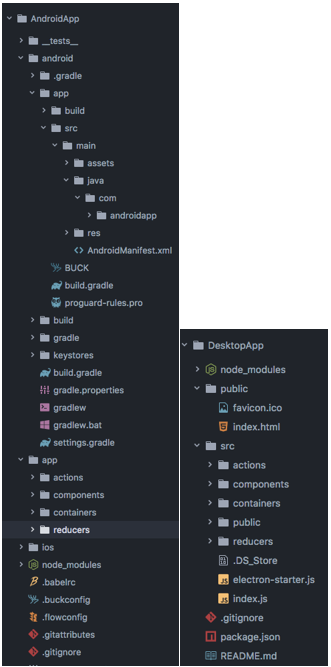
\includegraphics[scale=1]{pic8}
 
\end{figure}\\
\vspace{5mm}
The file structure is very similar to a standard React project with the exception of platform specific code being housed in the Android or ios folders.\\
\vspace{5mm}
Work on the application was going smoothly, considering my lack of experience, but due to the speed the rest of my group members were completing other portions of the project, I've now switched to developing the desktop application so we could more quickly begin integrating all the pieces together.\\
\vspace{5mm}
I ended up using my second choice in the tech document for the desktop application. Due to time constraints I needed to have as much code/logic re-usability as possible between the two applications so I chose to use React with Electron. The design patterns and logic in React are almost entirely interchangeable with React-Native. Because of this interchangeability I can write the entire desktop application and port the majority of my code over the mobile application with minimal code changes. This also gives the benefit of not having to learn an entire new language/ui framework because I'm already somewhat familiar with React. \\
\vspace{5mm}
I've discovered a ui framework called Material-UI which follows Google's Material UI design specification. It has both a React and React-Native implementation which are very similar and I've managed to get the library working with both applications. I also found a library called Redux which I can use to manage my applications state. I've updated my section of the tech document to include both these changes.\\
\vspace{5mm}
\begin{figure}[h!]
  
  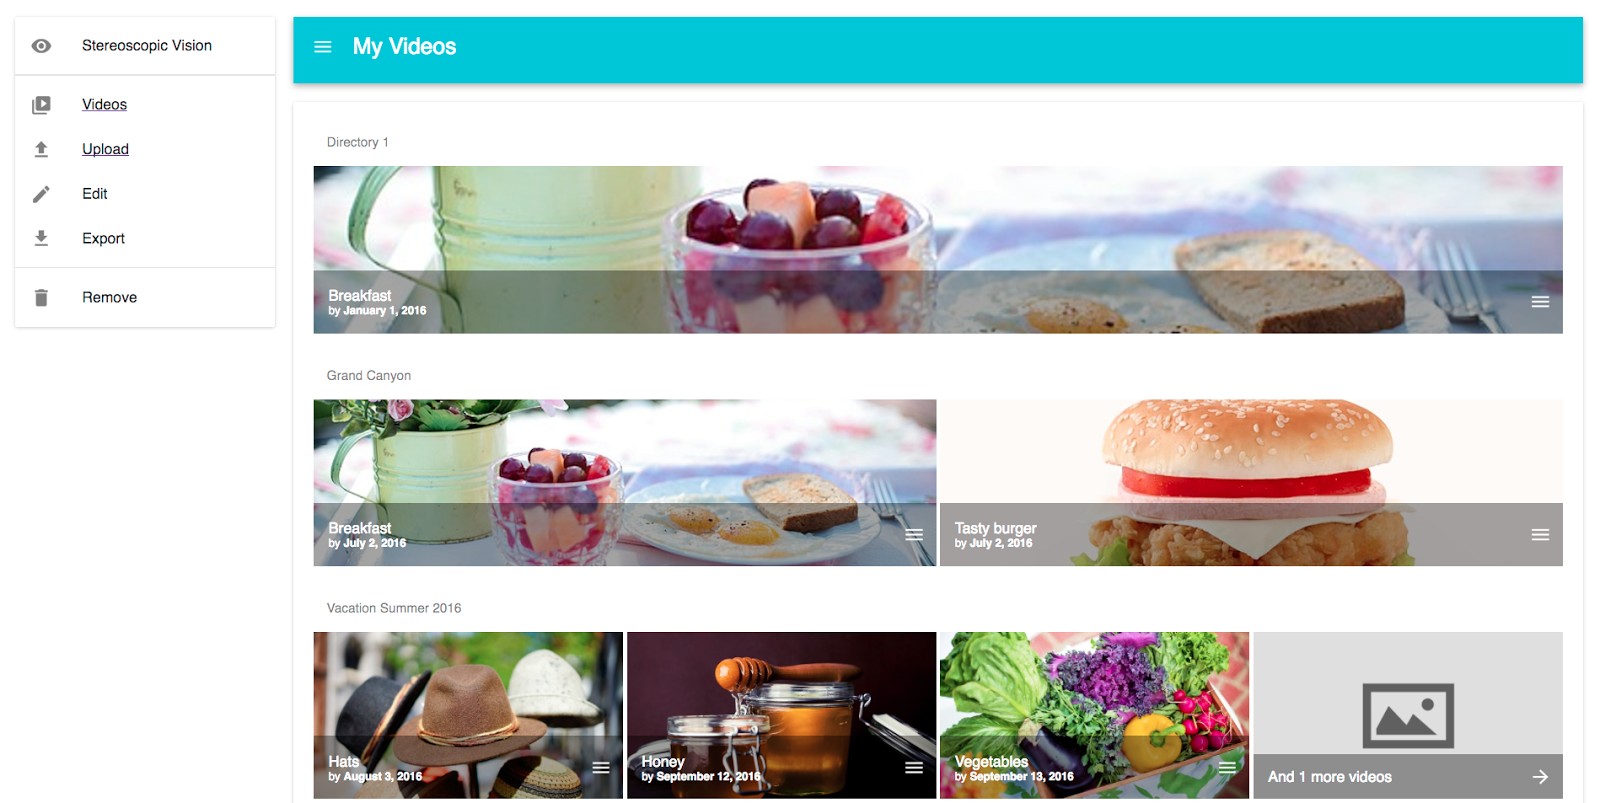
\includegraphics[scale=.4]{pic9}
  \caption{An example of what the UI will look like}
\end{figure}\\
\vspace{5mm}
In addition to working on the applications I set up a small debian server for our team to share files through and offset some of our file processing to. The hardware was provided by Kevin McGrath and setting it up was pretty straight forward. I had some trouble with the server denying remote ssh connections, but I was able to solve it by modifying the iptables configuration to allow external traffic to and from our ssh port.\\
\vspace{5mm}
Set up my development environments for both the desktop and mobile applications, created a basic home screen and menu for the mobile application, integrated a UI library and state management library into both my mobile and desktop applications, created the video file browser for the desktop application, created the file upload page for the desktop application, and set up a small file sharing/processing server for our group to use

\vspace{5mm}
{\Large\textbf{4.2 Problems that have come up}}\\
\vspace{5mm}
The biggest impediment that I've run into so far is the lack of time I have to put into the project. The past two terms I've had the largest workload I've ever had at school. I took the summer off my job to go on an internship and a lot of work has piled up that I've had to complete since I've come back. I try to allocate as much possible free time as I can to develop my portions of the project, but there is only so much time in the day. To try and counter this I've created a very strict calendar with time slots dedicated to project development. The dedicated time combined with the structure the calendar provides to other aspects of my life has been extremely helpful. \\
\vspace{5mm}
I haven't had much code trouble with my sections. The hardest issue I've had to overcome so far is getting the video file select function in my code to accept both directories and individual files and adjust the requirements of what the user has to upload based off that. For example if the user selects a single video file, the validation functions make sure to require an additional .FIT file to be selected as well. Overall working with the files on the user system vs. a server is a bit different than what I'm used to, with my background being primarily web application development.\\
\vspace{5mm}
{\Large\textbf{4.3 What I have left to do}}\\
\vspace{5mm}
I still have several screens to create for the desktop application and all but one screen for the Android application. On top of that I have to work with the frameworks I'm using to figure out how to call the functions my group mates are writing for the other parts of the project. I think this will be my biggest challenge so I'm looking to get started on that as soon as I flesh out the UI to a more usable state. I also need to find a database solution to hold information about the videos we process. I'm looking for one that can be used in both the Android and desktop application if possible. Once I finish completing those remaining tasks I'll have finished the sections of the project I was designated responsible for.\\
\vspace{5mm}
{\Large\textbf{5 Conclusion}}\\
\vspace{5mm}
Overall this term, we have made a lot of progress on our project. If we are able to keep up the progress we have been making, we should have a working product by the time Winter term is over. There might be a few bugs that are still problematic, but our applications should be completed on time. \\
\vspace{5mm}
{\Large\textbf{6 Bibliography}}\\
\vspace{5mm}
[1] ‘FIT SDK 20.22.00’, 2017. [Online]. Available:\\ https://www.thisisant.com/resources/fit. [Accessed: 14- Feb- 2017].\\
\vspace{5mm}
[2] NGHIAHO12, ‘videostab.cpp’, 2014. [Online]. Available:\\
http://nghiaho.com/uploads/code/videostab.cpp. [Accessed: 13- Feb- 2017].\\
\end{document}
